In \cite{clea07}, we already showed that SVMs clearly outperforms a
simple decision tree in solving the problem. Morover, it was therein
noted that the standard measure of performance for a SVM classifier
(the fraction of correctly guessed labels over the total number of
samples) is biased, at least in two ways: firstly, the number of $1$
labels is much smaller than that of $-1$ labels; as a consequence, a
dumb predictor which guessed $-1$ identically would achieve an average
accuracy of about $83\%$. Therefore we adopt a weigthed measure of
accuracy, $\frac{n_{-1} c_1 + n_1 c_{-1}}{c_1+c_{-1}}$, where $n_i$ is
the number of correctly guessed $i$ labels, $i \in \{1,-1\}$, and
$c_i$ is the total number of $i$ labels.

Secondly, we are looking for both accurate \emph{and small} models;
this means that looking for the most accurate models could lead to
unnecessarily large models --- this fact was also shown in
\cite{clea07}. Therefore, we adopt here an index of performance given
by the ratio of the weighted accuracy detailed above and the
percentage of support vectors in the obtained model. This index was
used for grid searching the best values of $C$ and $\sigma$.

Figure \ref{fig:comparison} shows the weighted accuracy and size of
the obtained models as $T_c$ is increased, both when using and not
using the gaze.

\begin{figure}[!ht]
  \centering
    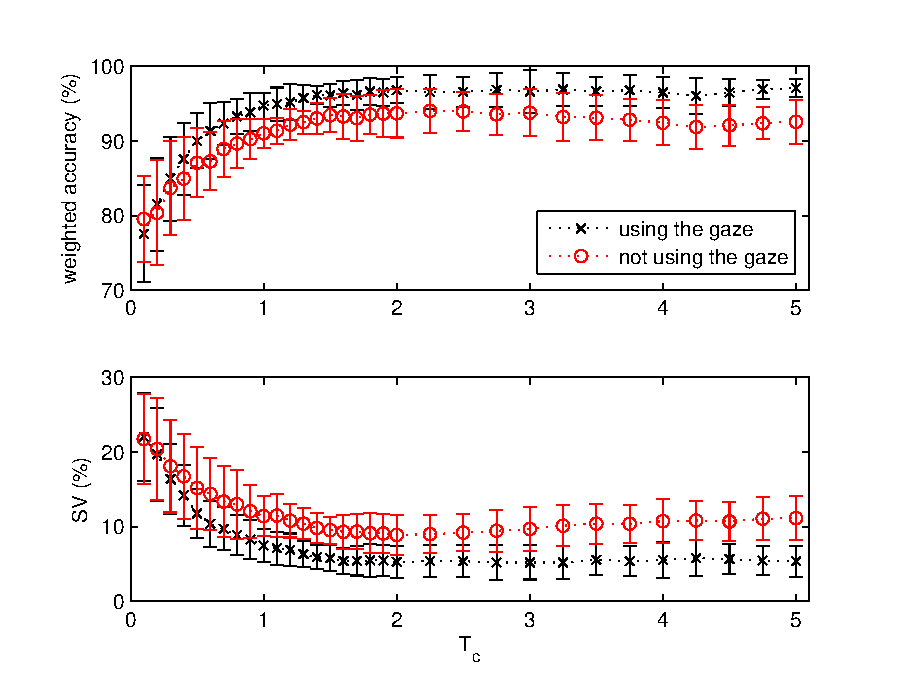
\includegraphics[width=\linewidth]{figs/comparison.eps}
    \caption{Comparison between not using the gaze (red curve) and
    using the gaze (black one) as $T_c$ increases. Top panel: weighted
    accuracy. Bottom panel: size of the models, expressed as the
    fraction of Support Vectors. Dots are the mean values over all
    subjects, whereas the errorbars denote $\pm$ one standard deviation.}
    \label{fig:comparison}
\end{figure}

First of all, the effect predicted in the previous Section is present:
both the accuracy and size of the models become better as $T_c$ is
increased, and then they reach a maximum around $T_c=2$ seconds; then
they remain essentially constant. Secondly, notice that the use of the
gaze uniformly and consistently improves both the accuracy of the
models and their size, the black curve being systematically higher
than the red one, as far as the accuracy is concerned, and lower in
the case of the model size. From $T_c\geq 2$, there is little overlap
among the errorbars, indicating a stastically significant
improvement. Thirdly, it seems that such a value of $T_c$ is just
about right for all subjects, notwithstanding their differences; this
could dramatically reduce the setup time in a real setting.

For $T_c=2$ seconds, the accuracy is $96.79\% \pm 1.7\%$ using the
gaze, as opposed to $93.69\% \pm 3.24\%$ when not using it; the model
size is $5.27\% \pm 2.12\%$ as opposed to $8.88\% \pm 2.73\%$. The
mean values are better, and the standard deviations are smaller when
using the gaze, denoting better performance and higher robustness with
respect to the diversity of the subjects.

Let us then turn to the experiment with the gaze, and analyse the
performance in deeper detail for the single subjects. Figure
\ref{fig:subjects} shows the same results as the black curves of Figure
\ref{fig:comparison}, but for each subject.

\begin{figure*}[!ht]
  \centering
    \begin{tabular}{cc}
      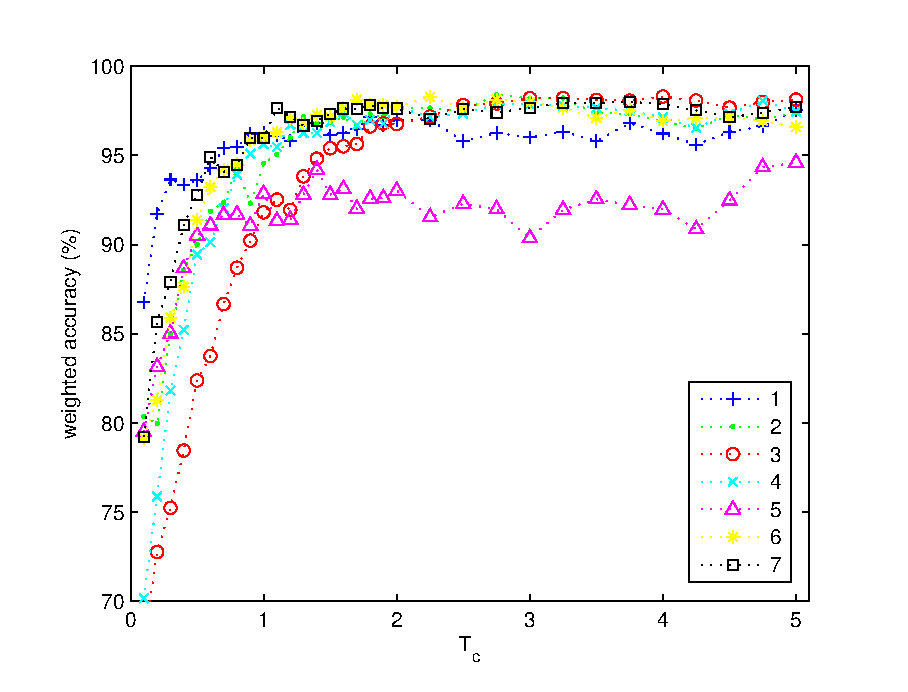
\includegraphics[width=0.45\textwidth]{figs/subjects_acc.eps} &
      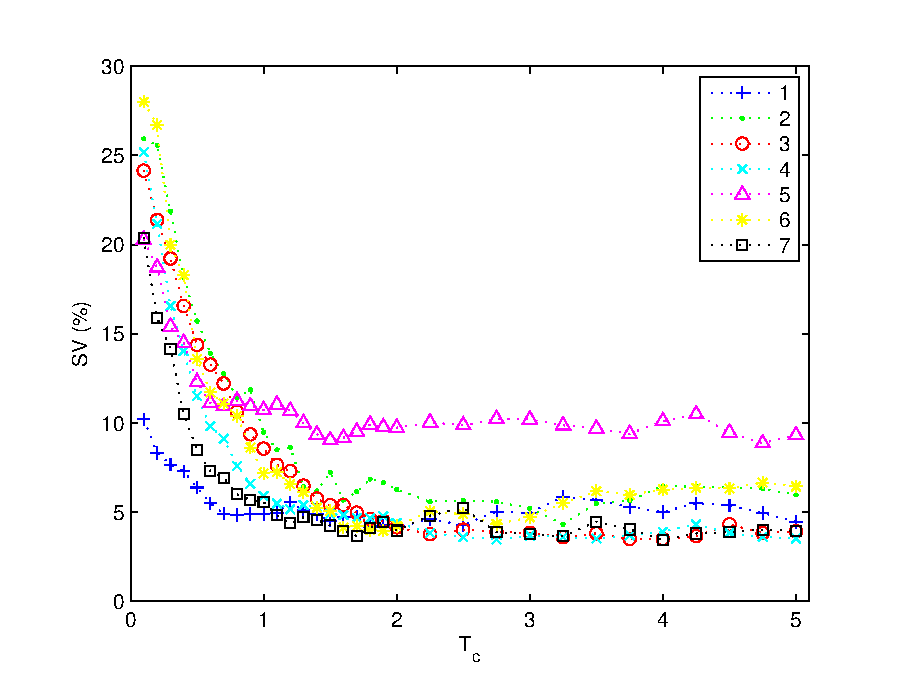
\includegraphics[width=0.45\textwidth]{figs/subjects_size.eps} \\
      $(a)$ & $(b)$
    \end{tabular}
    \caption{Accuracy $(a)$ and size $(b)$ of the models for each single subject,
    using the gaze.}
    \label{fig:subjects}
\end{figure*}

Consider the Figure, pane $(a)$: it is apparent that the worst subject
is number $5$, a 73-years old woman who has undergone in
the past a cataract surgical operation. It is not surprising that this
is the hardest subject; still, for $T_c=2$, the model has a remarkable
accuracy of $93.03\%$. All other subjects reach an accuracy of
$96.75\%$ and more for the same value of $T_c$. Analogous
considerations apply as far as the model size is concerned (pane $(b)$
of the same Figure). It is interesting to note that, even for such a
hard subject as subject $5$, the use of the gaze signal greatly
improves the accuracy of the model (see Figure \ref{fig:mama}).

\begin{figure}[!ht]
  \centering
    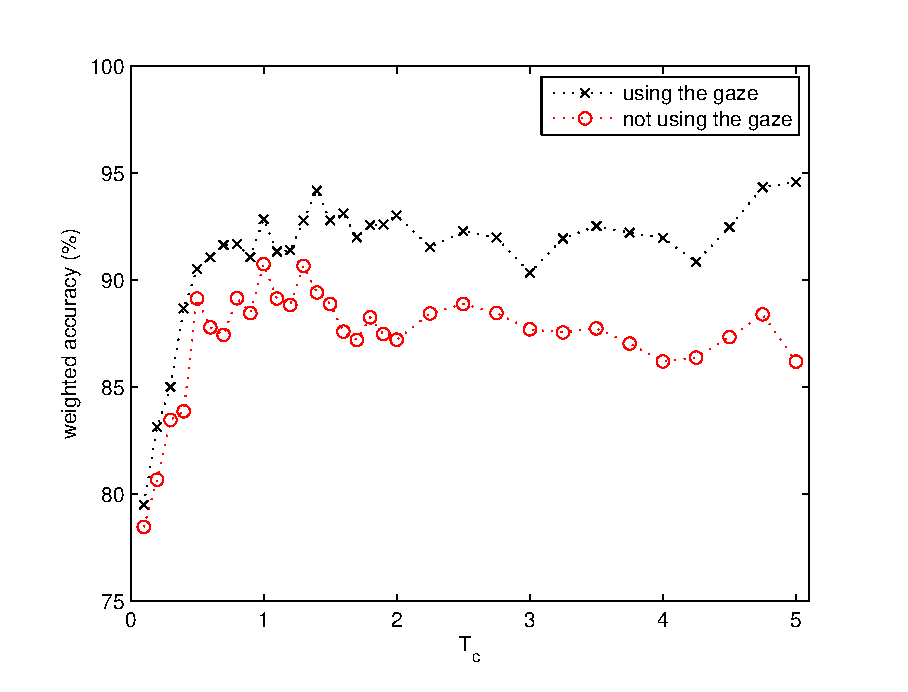
\includegraphics[width=\linewidth]{figs/mama.eps}
    \caption{Comparison between not using the gaze (red curve) and
    using the gaze (black one) as $T_c$ increases, for subject $5$.}
    \label{fig:mama}
\end{figure}
